% ============================================================
% Appendix C（倒産確率の等高線図 & 差分図）
% ============================================================

\chapter*{付録 C：倒産確率の等高線図および差分図}
\addcontentsline{toc}{chapter}{付録 C：倒産確率の等高線図および差分図}

本付録では，第6章で提示した倒産確率サーフェスの補足として，
各ケース（A〜F）の倒産確率 $p$ の等高線図（top view）を示す。
これにより，倒産境界線（$Z_{\text{lin}} = 0$）の形状や，
収益性 $\mu$ と市場ショック $\sigma$ の組み合わせが倒産確率に与える影響を
より直感的に把握できる。
さらに，構造的に意味のある 2 組の比較
（大企業 vs 地方電力，商社系 vs 地域新電力）
について，倒産確率の差分図を示し，
支援能力 $S$ および負債比率 $D$ の影響を定量的に確認する。

% ------------------------------------------------------------
\section*{C.1 ケース別等高線図（A〜F）}
\addcontentsline{toc}{section}{C.1 ケース別等高線図（A〜F）}

以下に，ケースA〜Fの倒産確率 $p$ の等高線図を示す。
いずれも $\mu \in [-0.10, 0.10]$，$\sigma \in [0.05, 0.50]$ の範囲で計算し，
倒産境界線（$Z_{\text{lin}} = 0$）を赤線で強調している。
倒産境界線の位置と形状を比較することで，
負債比率 $D$ と支援能力 $S$ が倒産リスクに与える影響を視覚的に理解できる。

\begin{figure}[H]
    \centering
    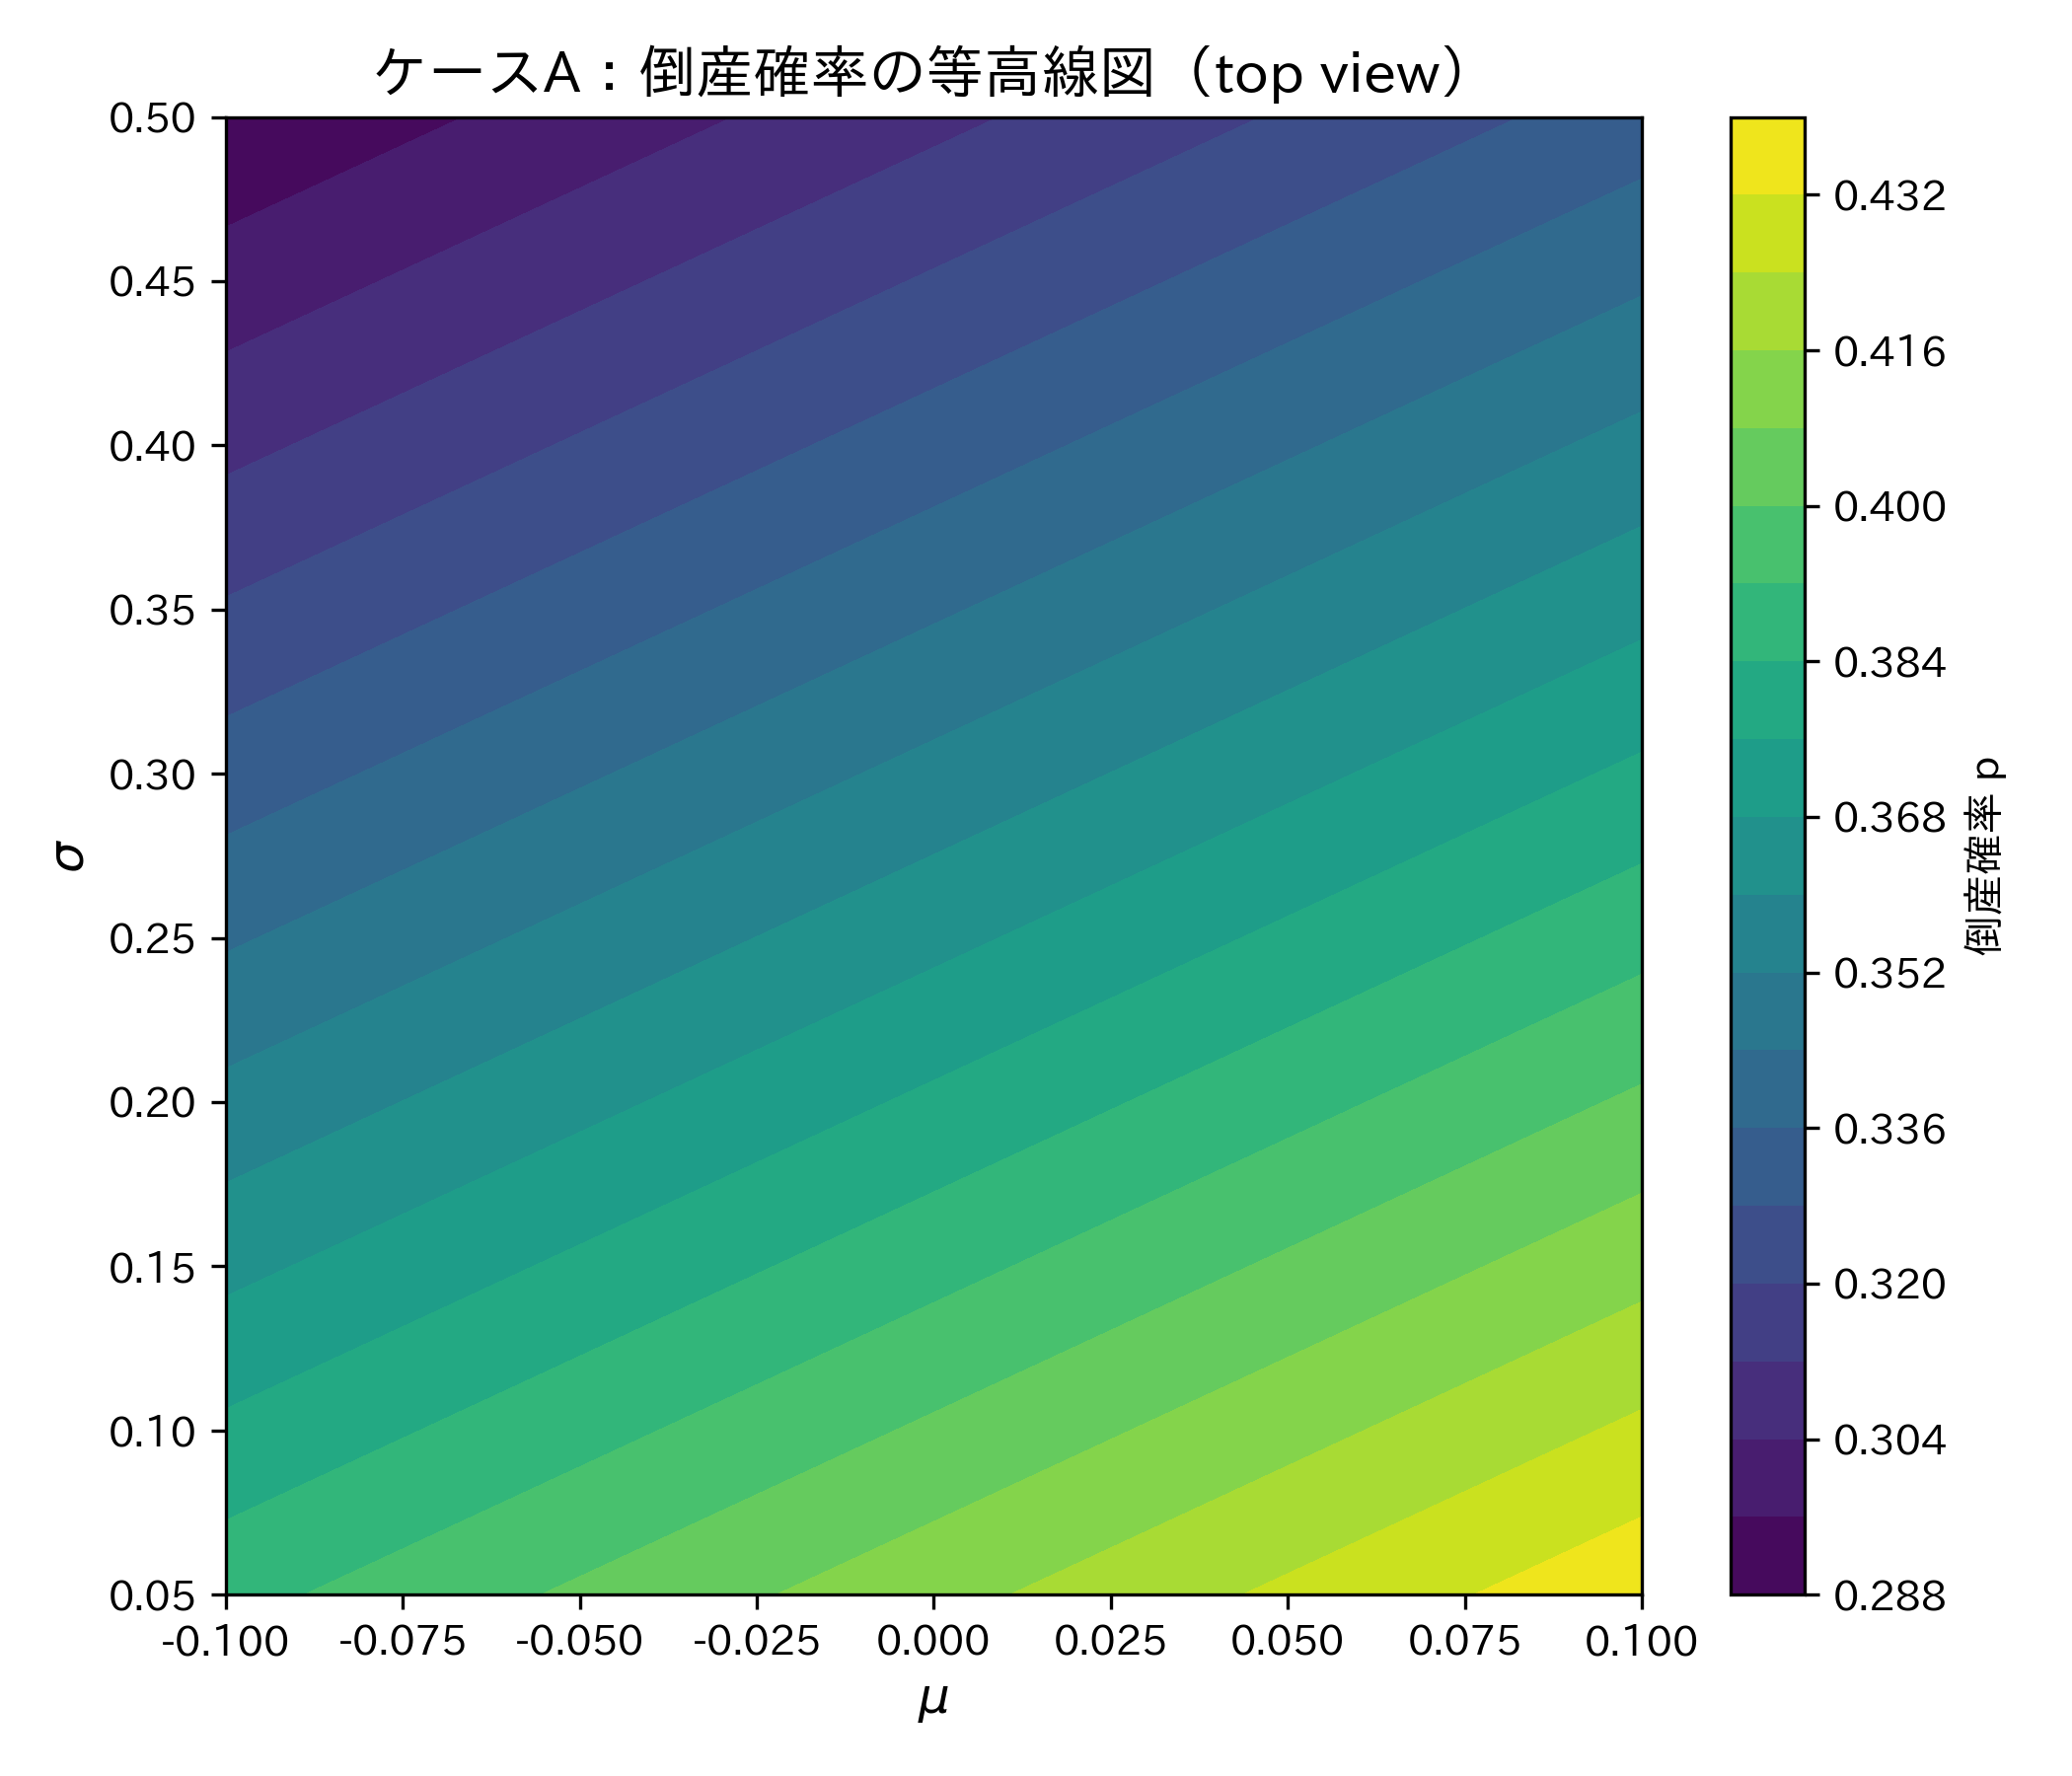
\includegraphics[width=0.75\linewidth]{figures/contour_caseA.png}
    \caption{ケースA（$D=0.3,\ S=0$）：倒産確率の等高線図。
    支援能力がなく，負債比率も低いため，境界線は中間的な位置にある。}
\end{figure}

\begin{figure}[H]
    \centering
    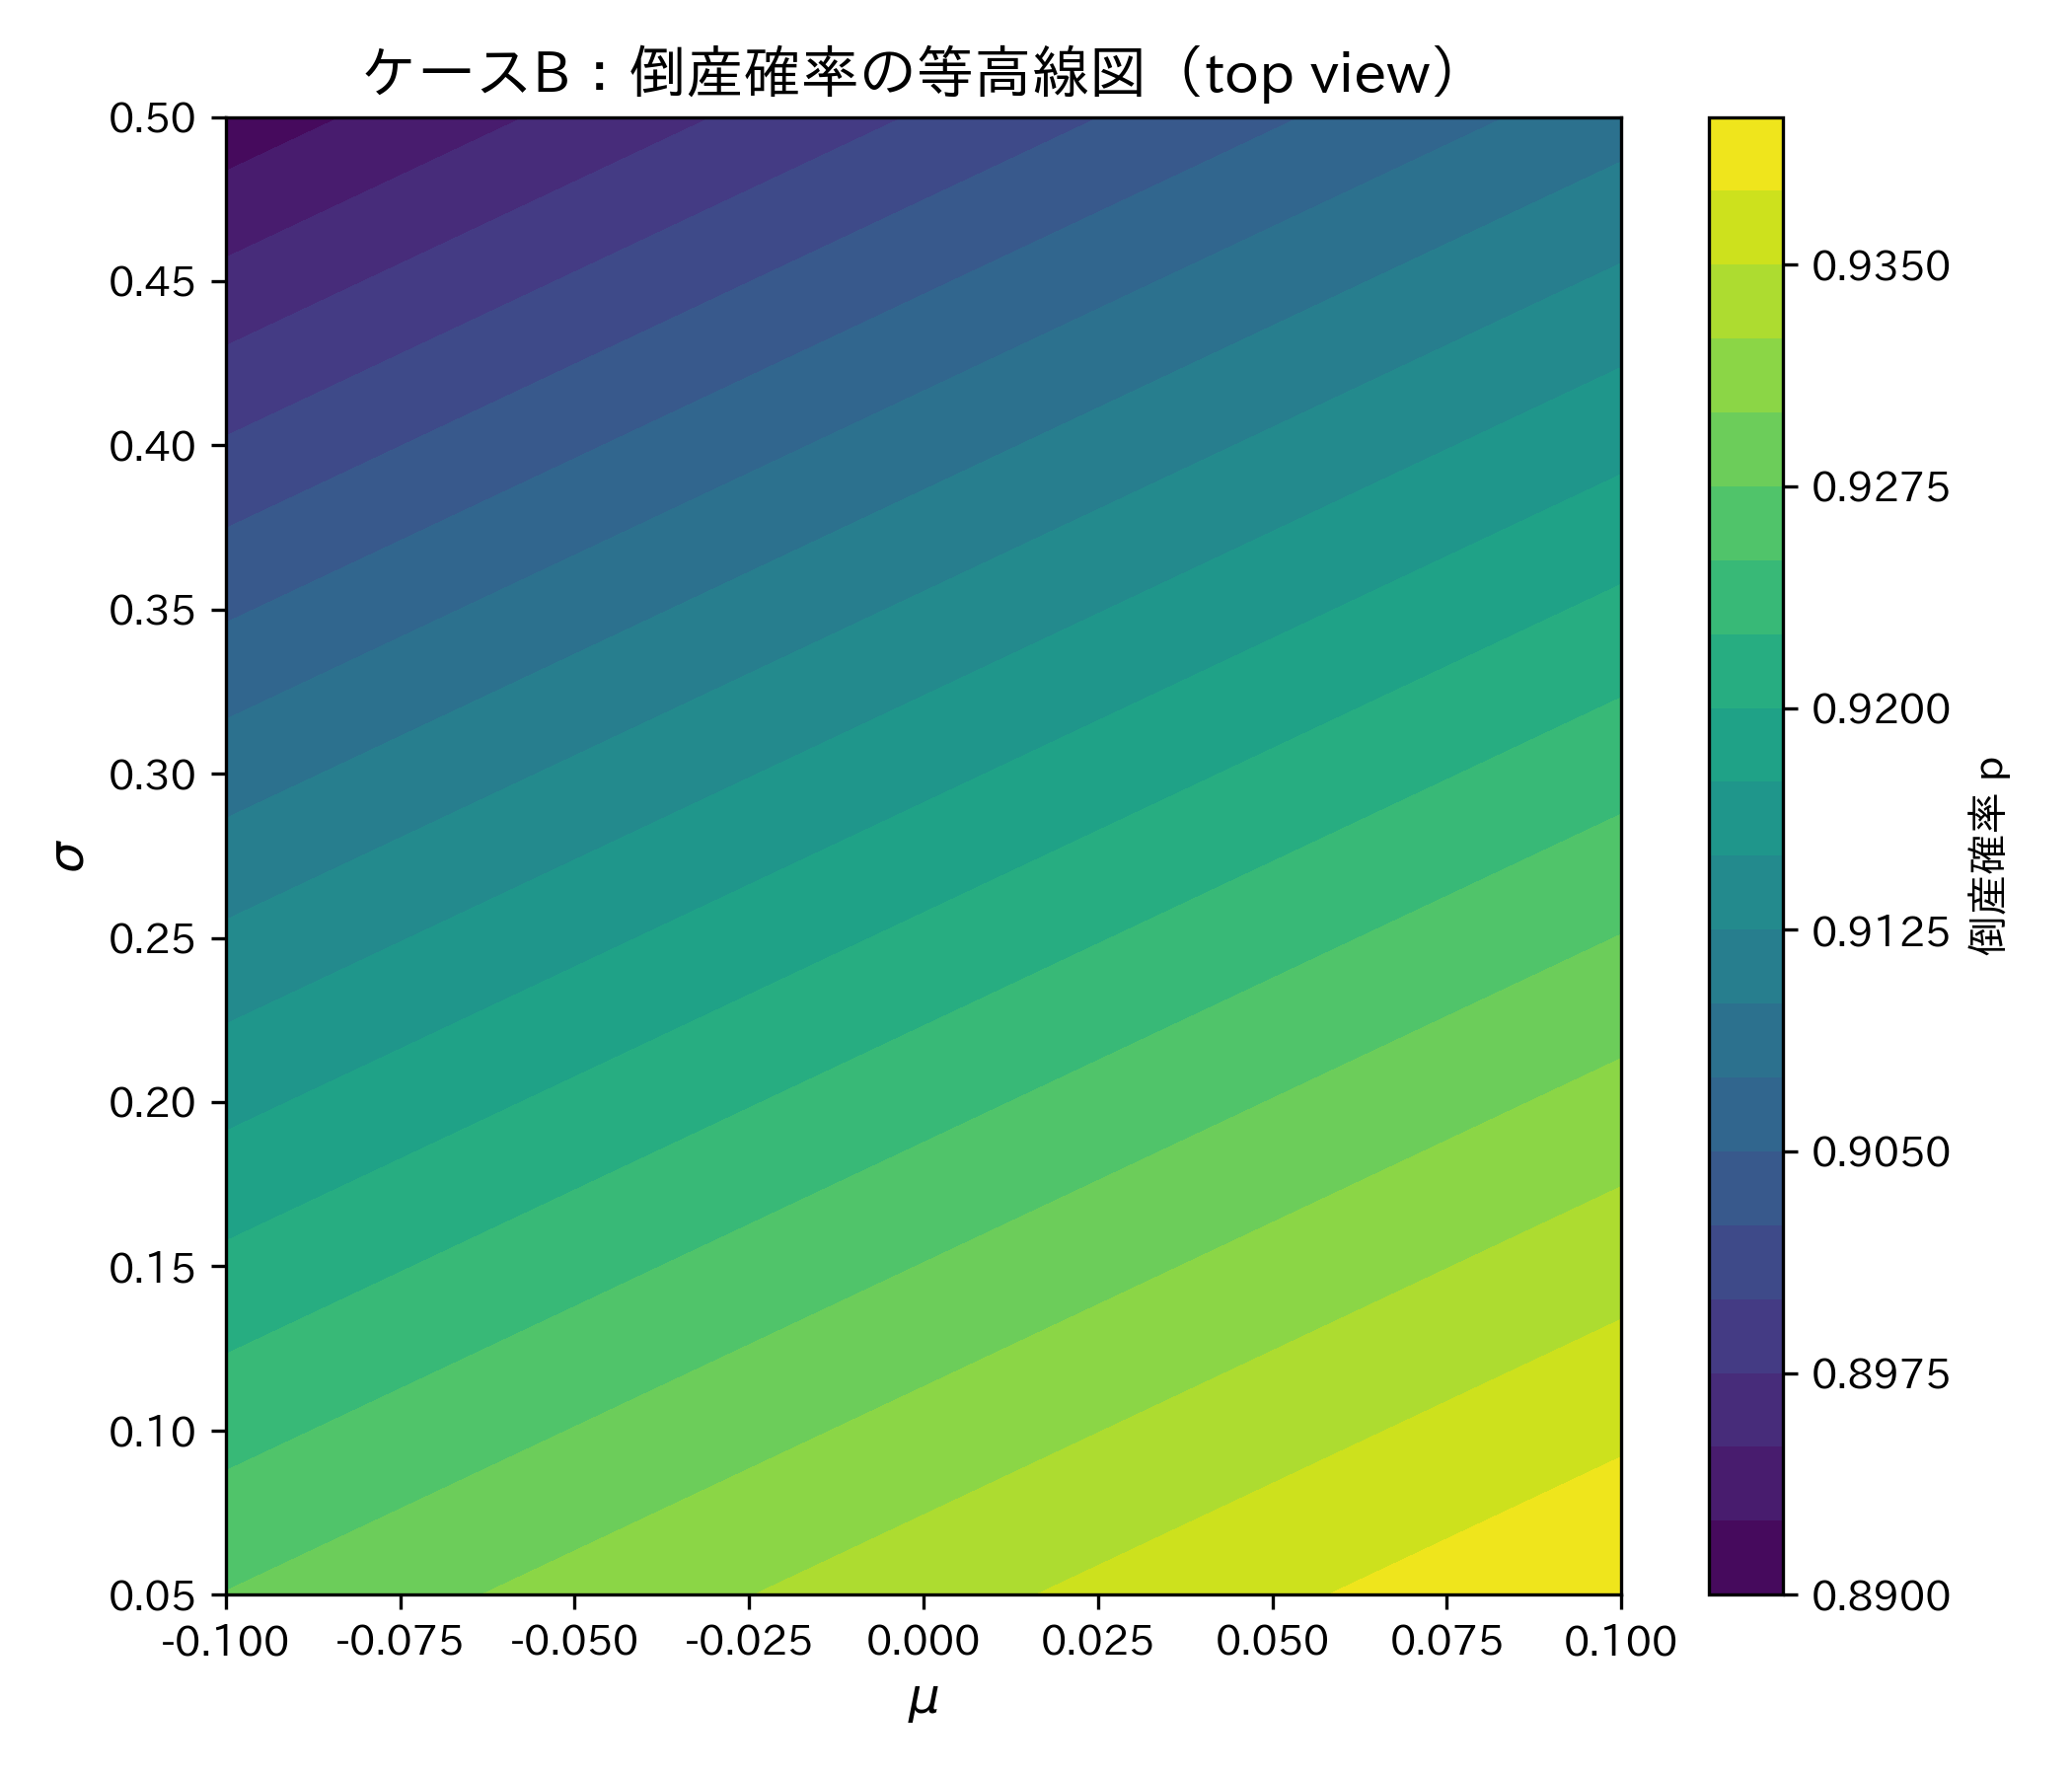
\includegraphics[width=0.75\linewidth]{figures/contour_caseB.png}
    \caption{ケースB（$D=0.3,\ S=3$）：倒産確率の等高線図。
    強い支援能力により倒産境界線が大きく右へ移動し，
    市場ショックに対する耐性が高いことがわかる。}
\end{figure}

\begin{figure}[H]
    \centering
    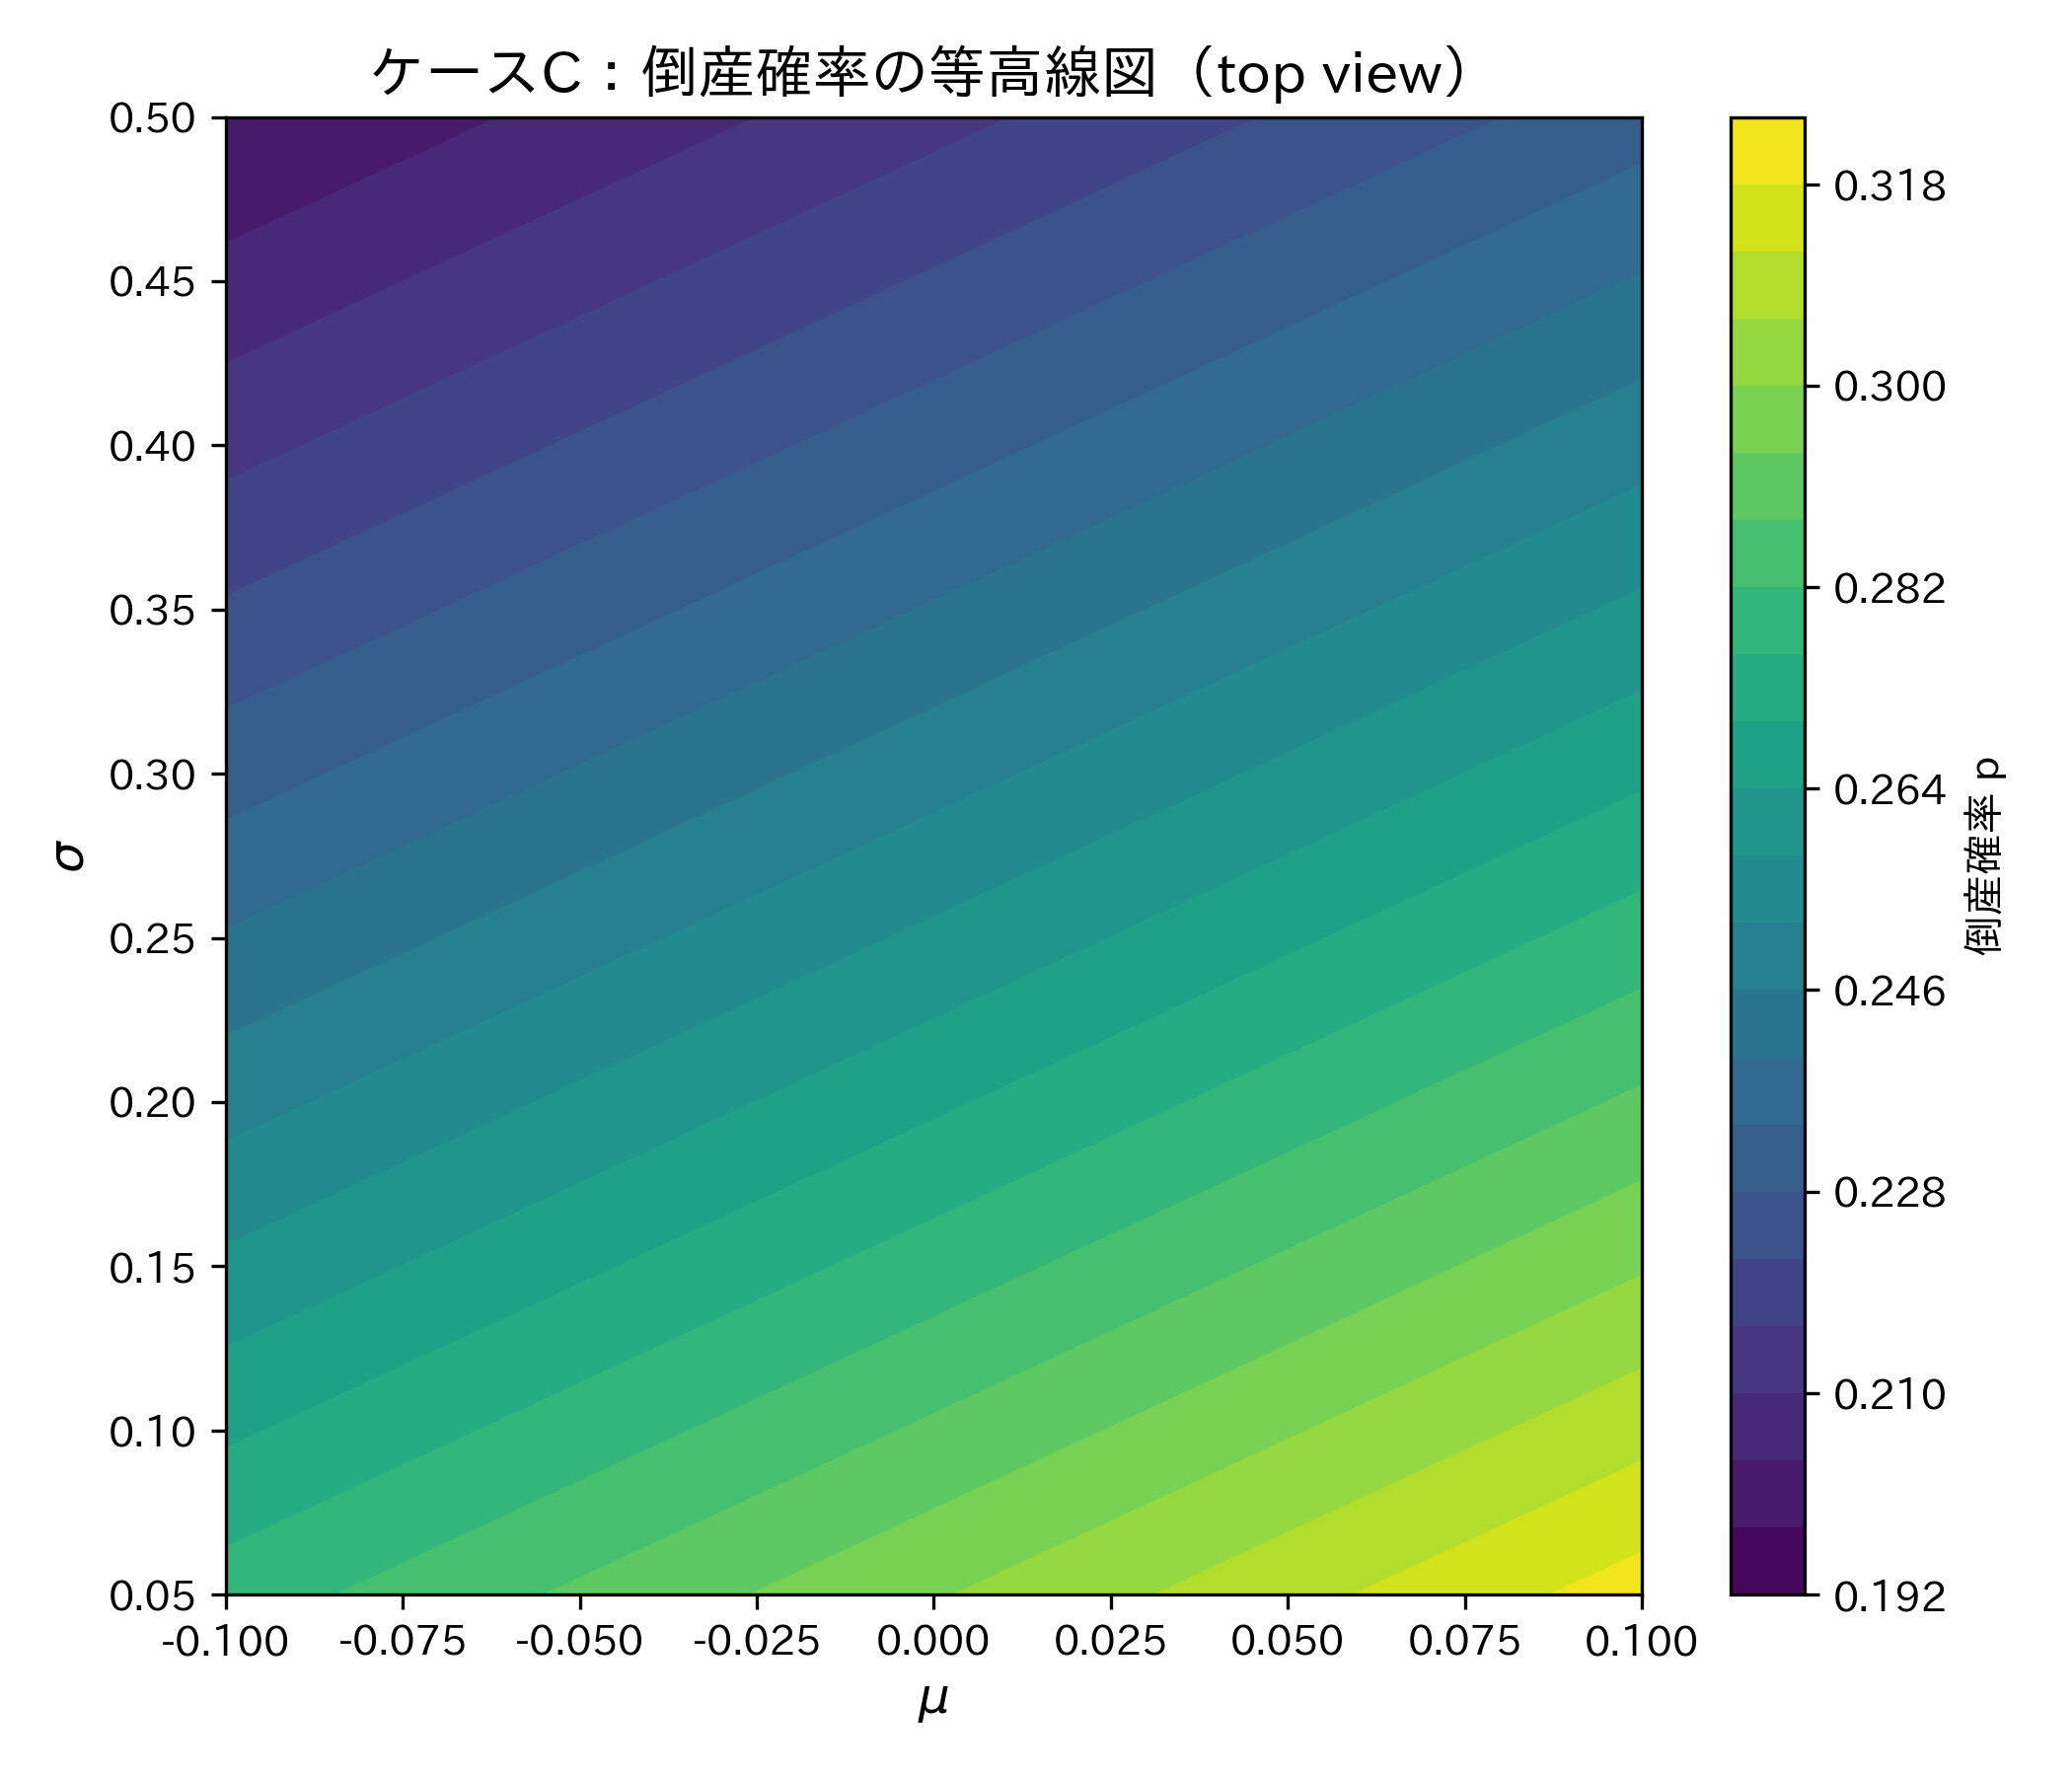
\includegraphics[width=0.75\linewidth]{figures/contour_caseC.png}
    \caption{ケースC（$D=0.8,\ S=0$）：倒産確率の等高線図。
    負債過多により境界線が大きく左へ寄り，
    高ボラティリティ環境で極めて脆弱であることが示される。}
\end{figure}

\begin{figure}[H]
    \centering
    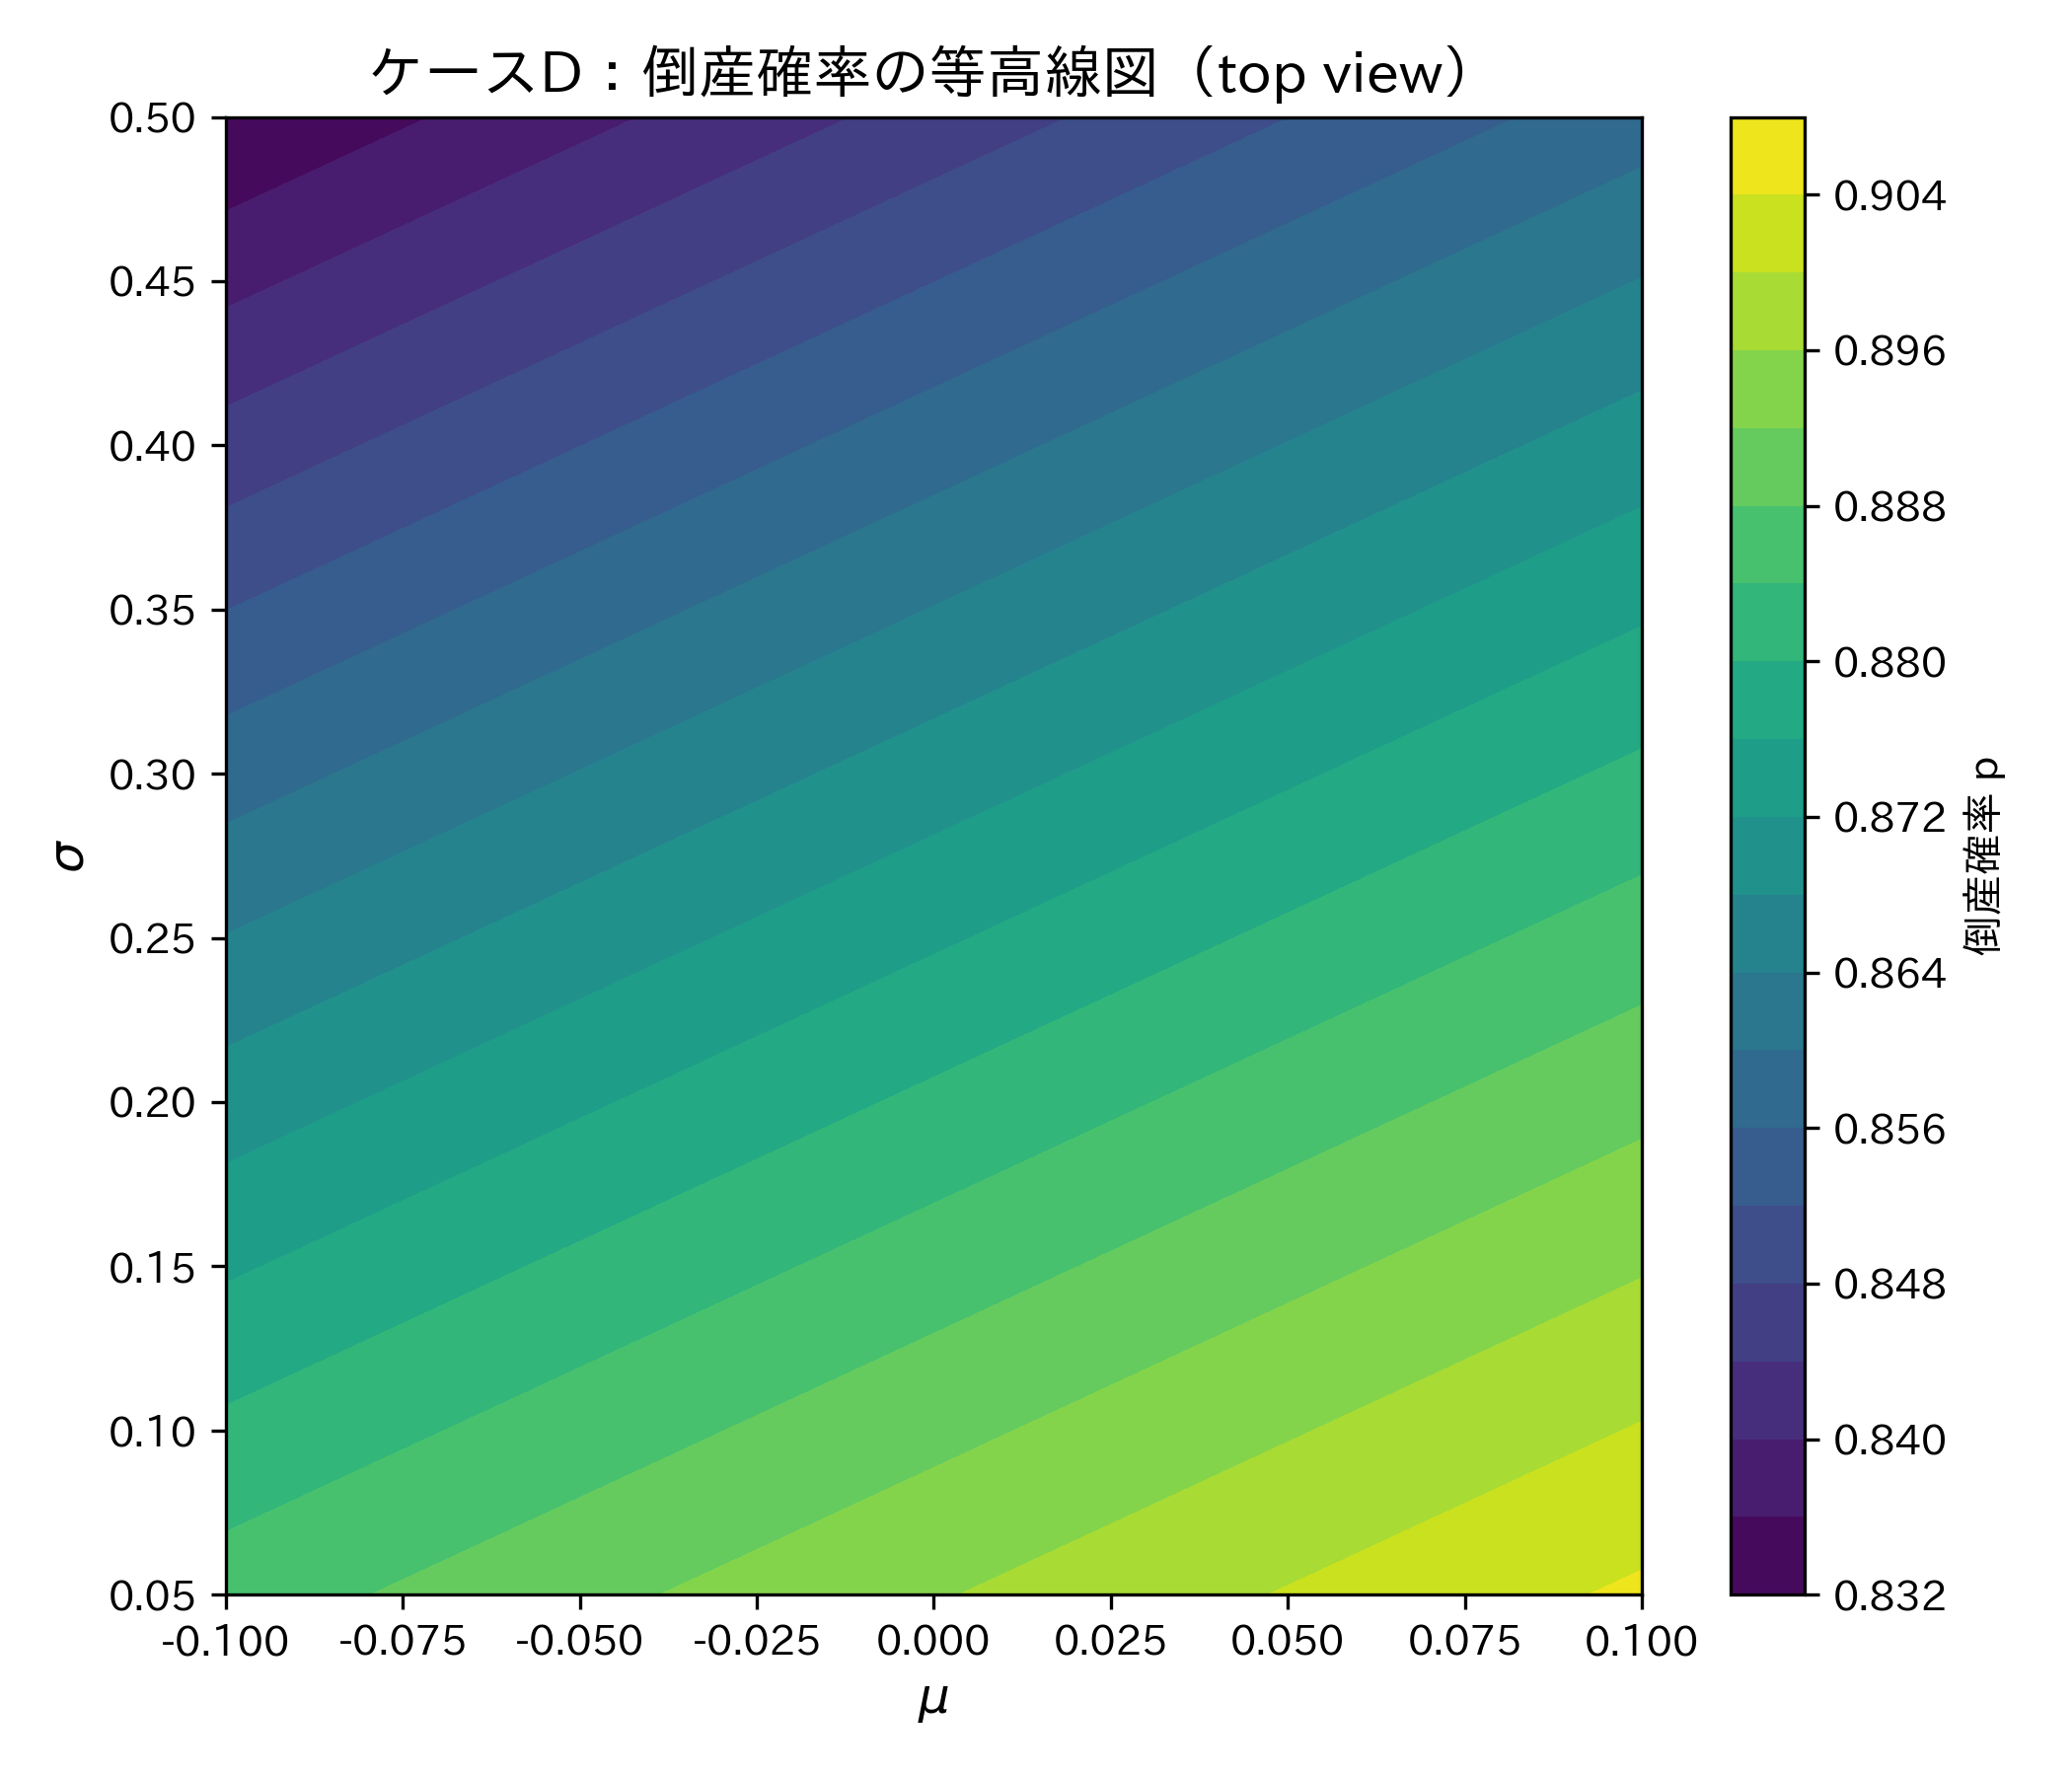
\includegraphics[width=0.75\linewidth]{figures/contour_caseD.png}
    \caption{ケースD（$D=0.8,\ S=3$）：倒産確率の等高線図。
    負債比率は高いが支援能力が強いため，
    ケースCと比べて境界線が右へ戻り，倒産リスクが大幅に緩和されている。}
\end{figure}

\begin{figure}[H]
    \centering
    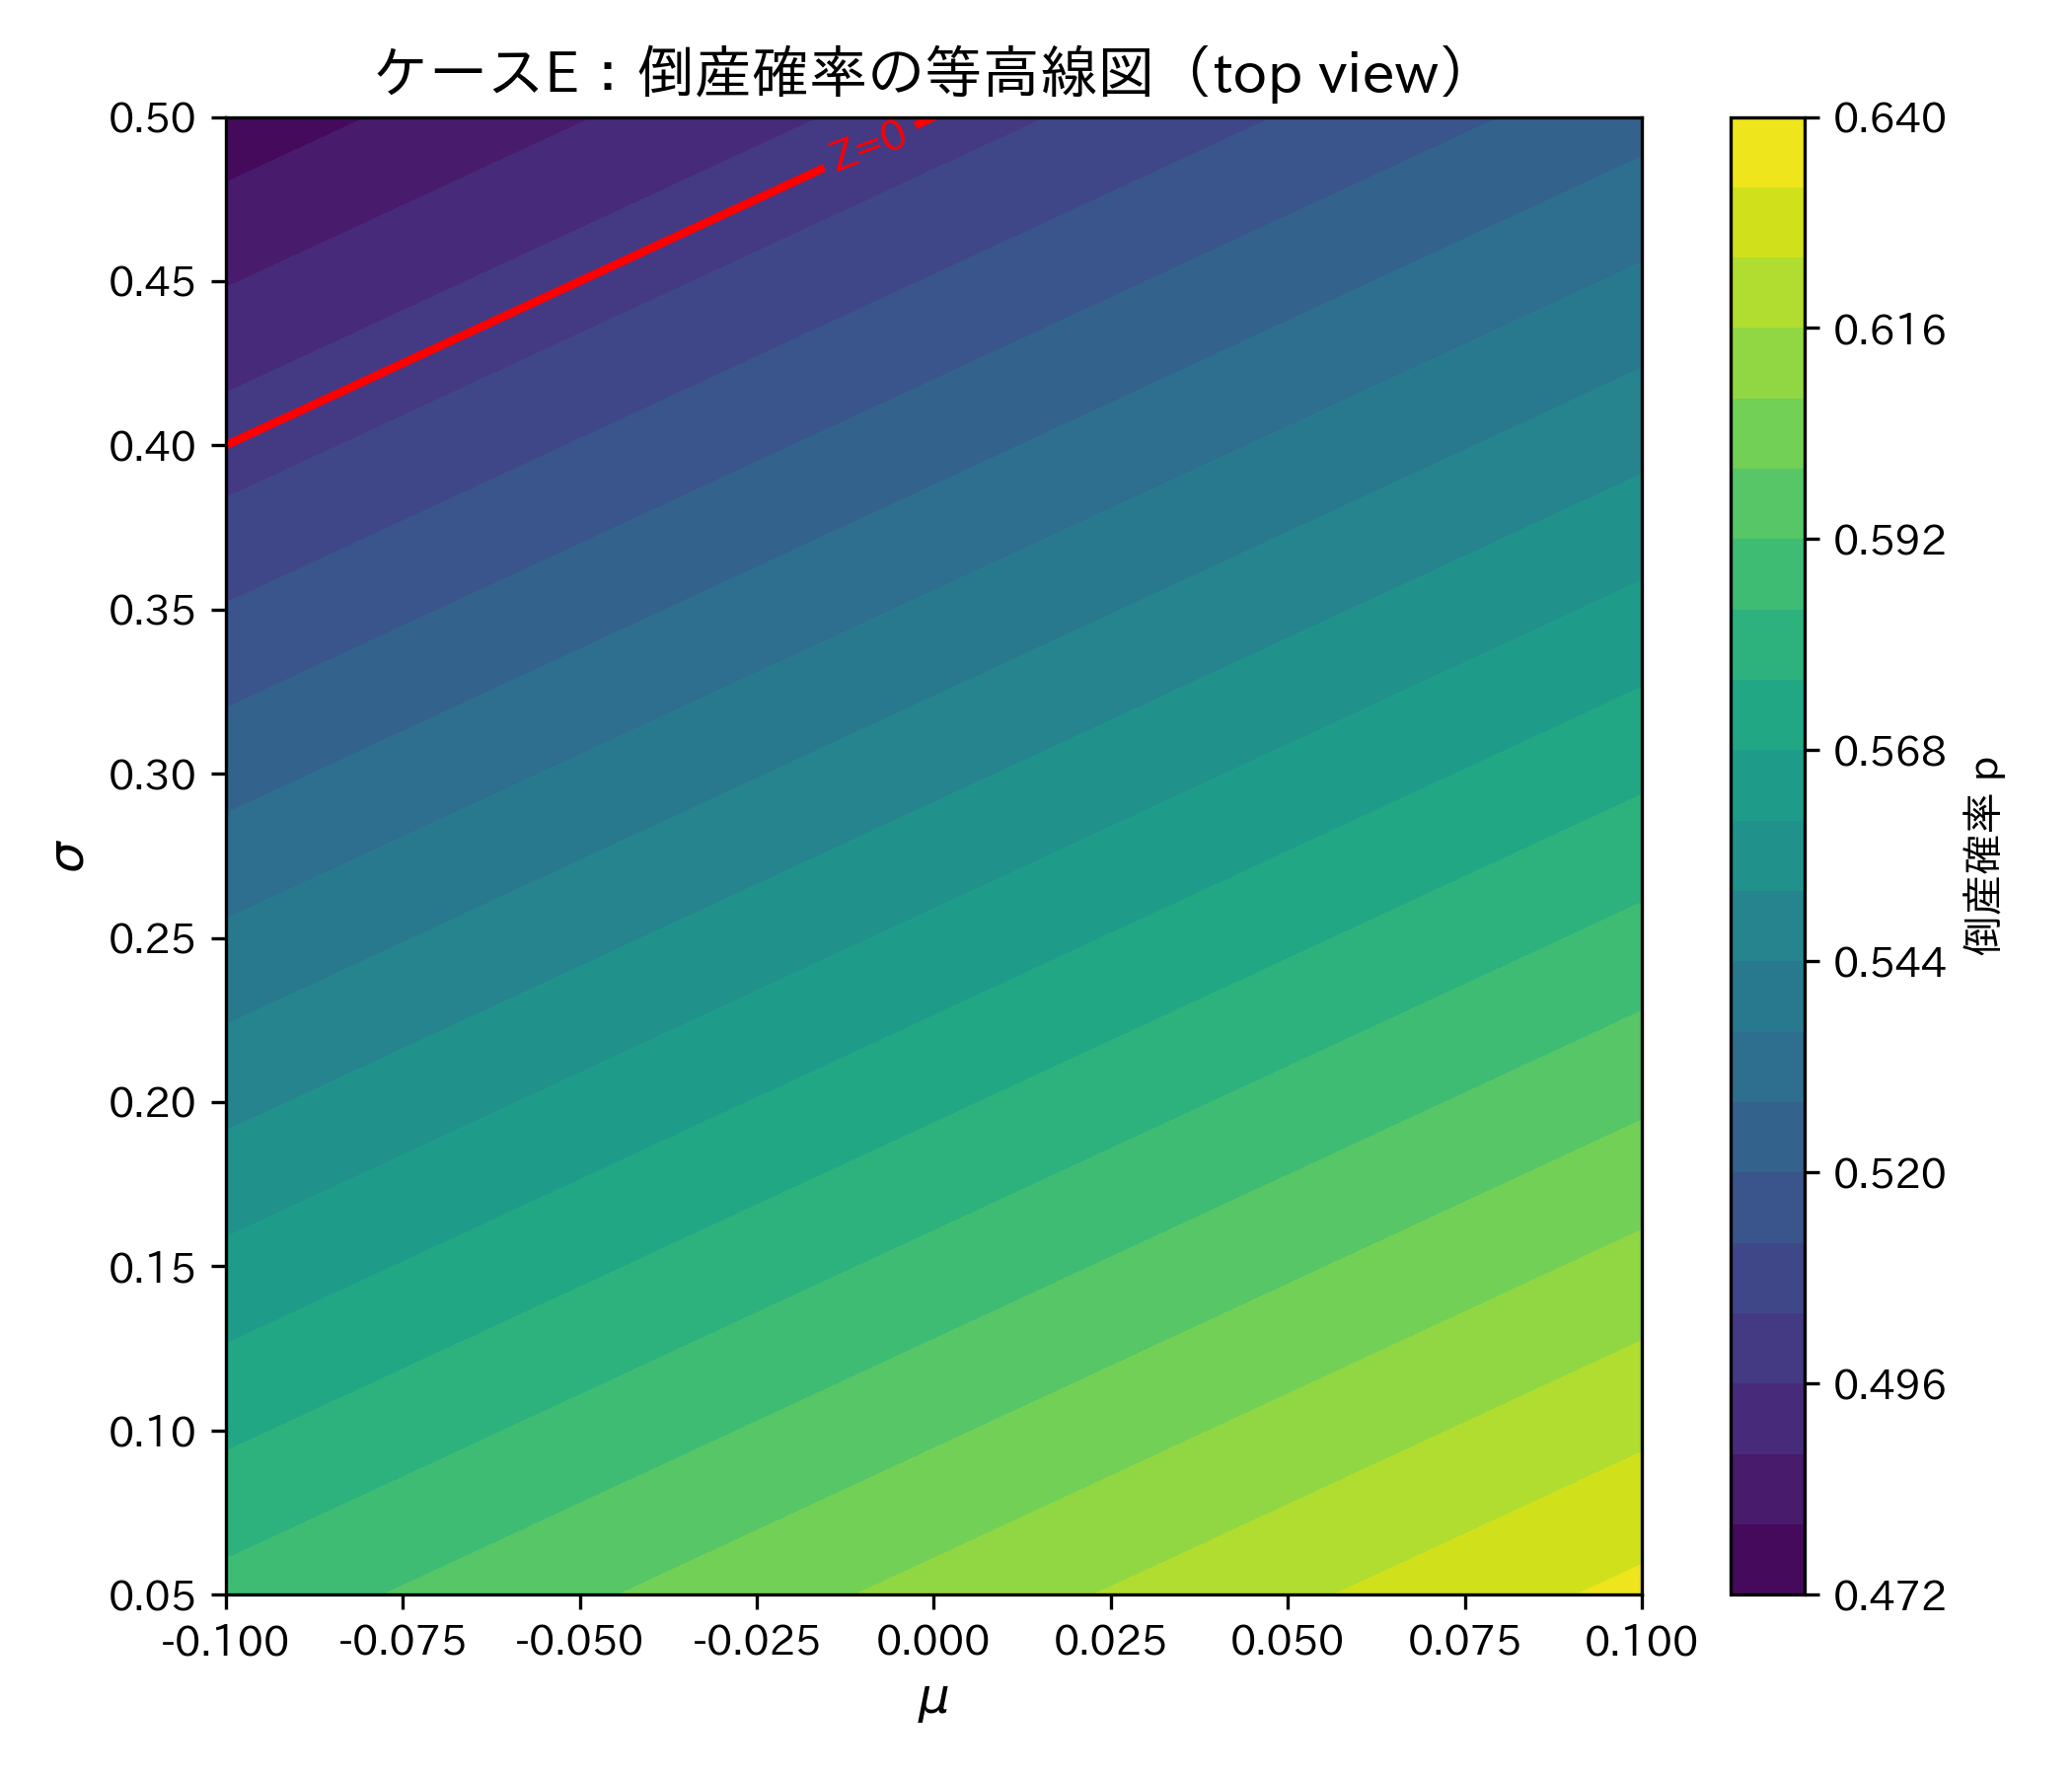
\includegraphics[width=0.75\linewidth]{figures/contour_caseE.png}
    \caption{ケースE（$D=0.5,\ S=1$）：倒産確率の等高線図。
    地域新電力の典型であり，収益性と市場ショックに敏感な構造が確認できる。}
\end{figure}

\begin{figure}[H]
    \centering
    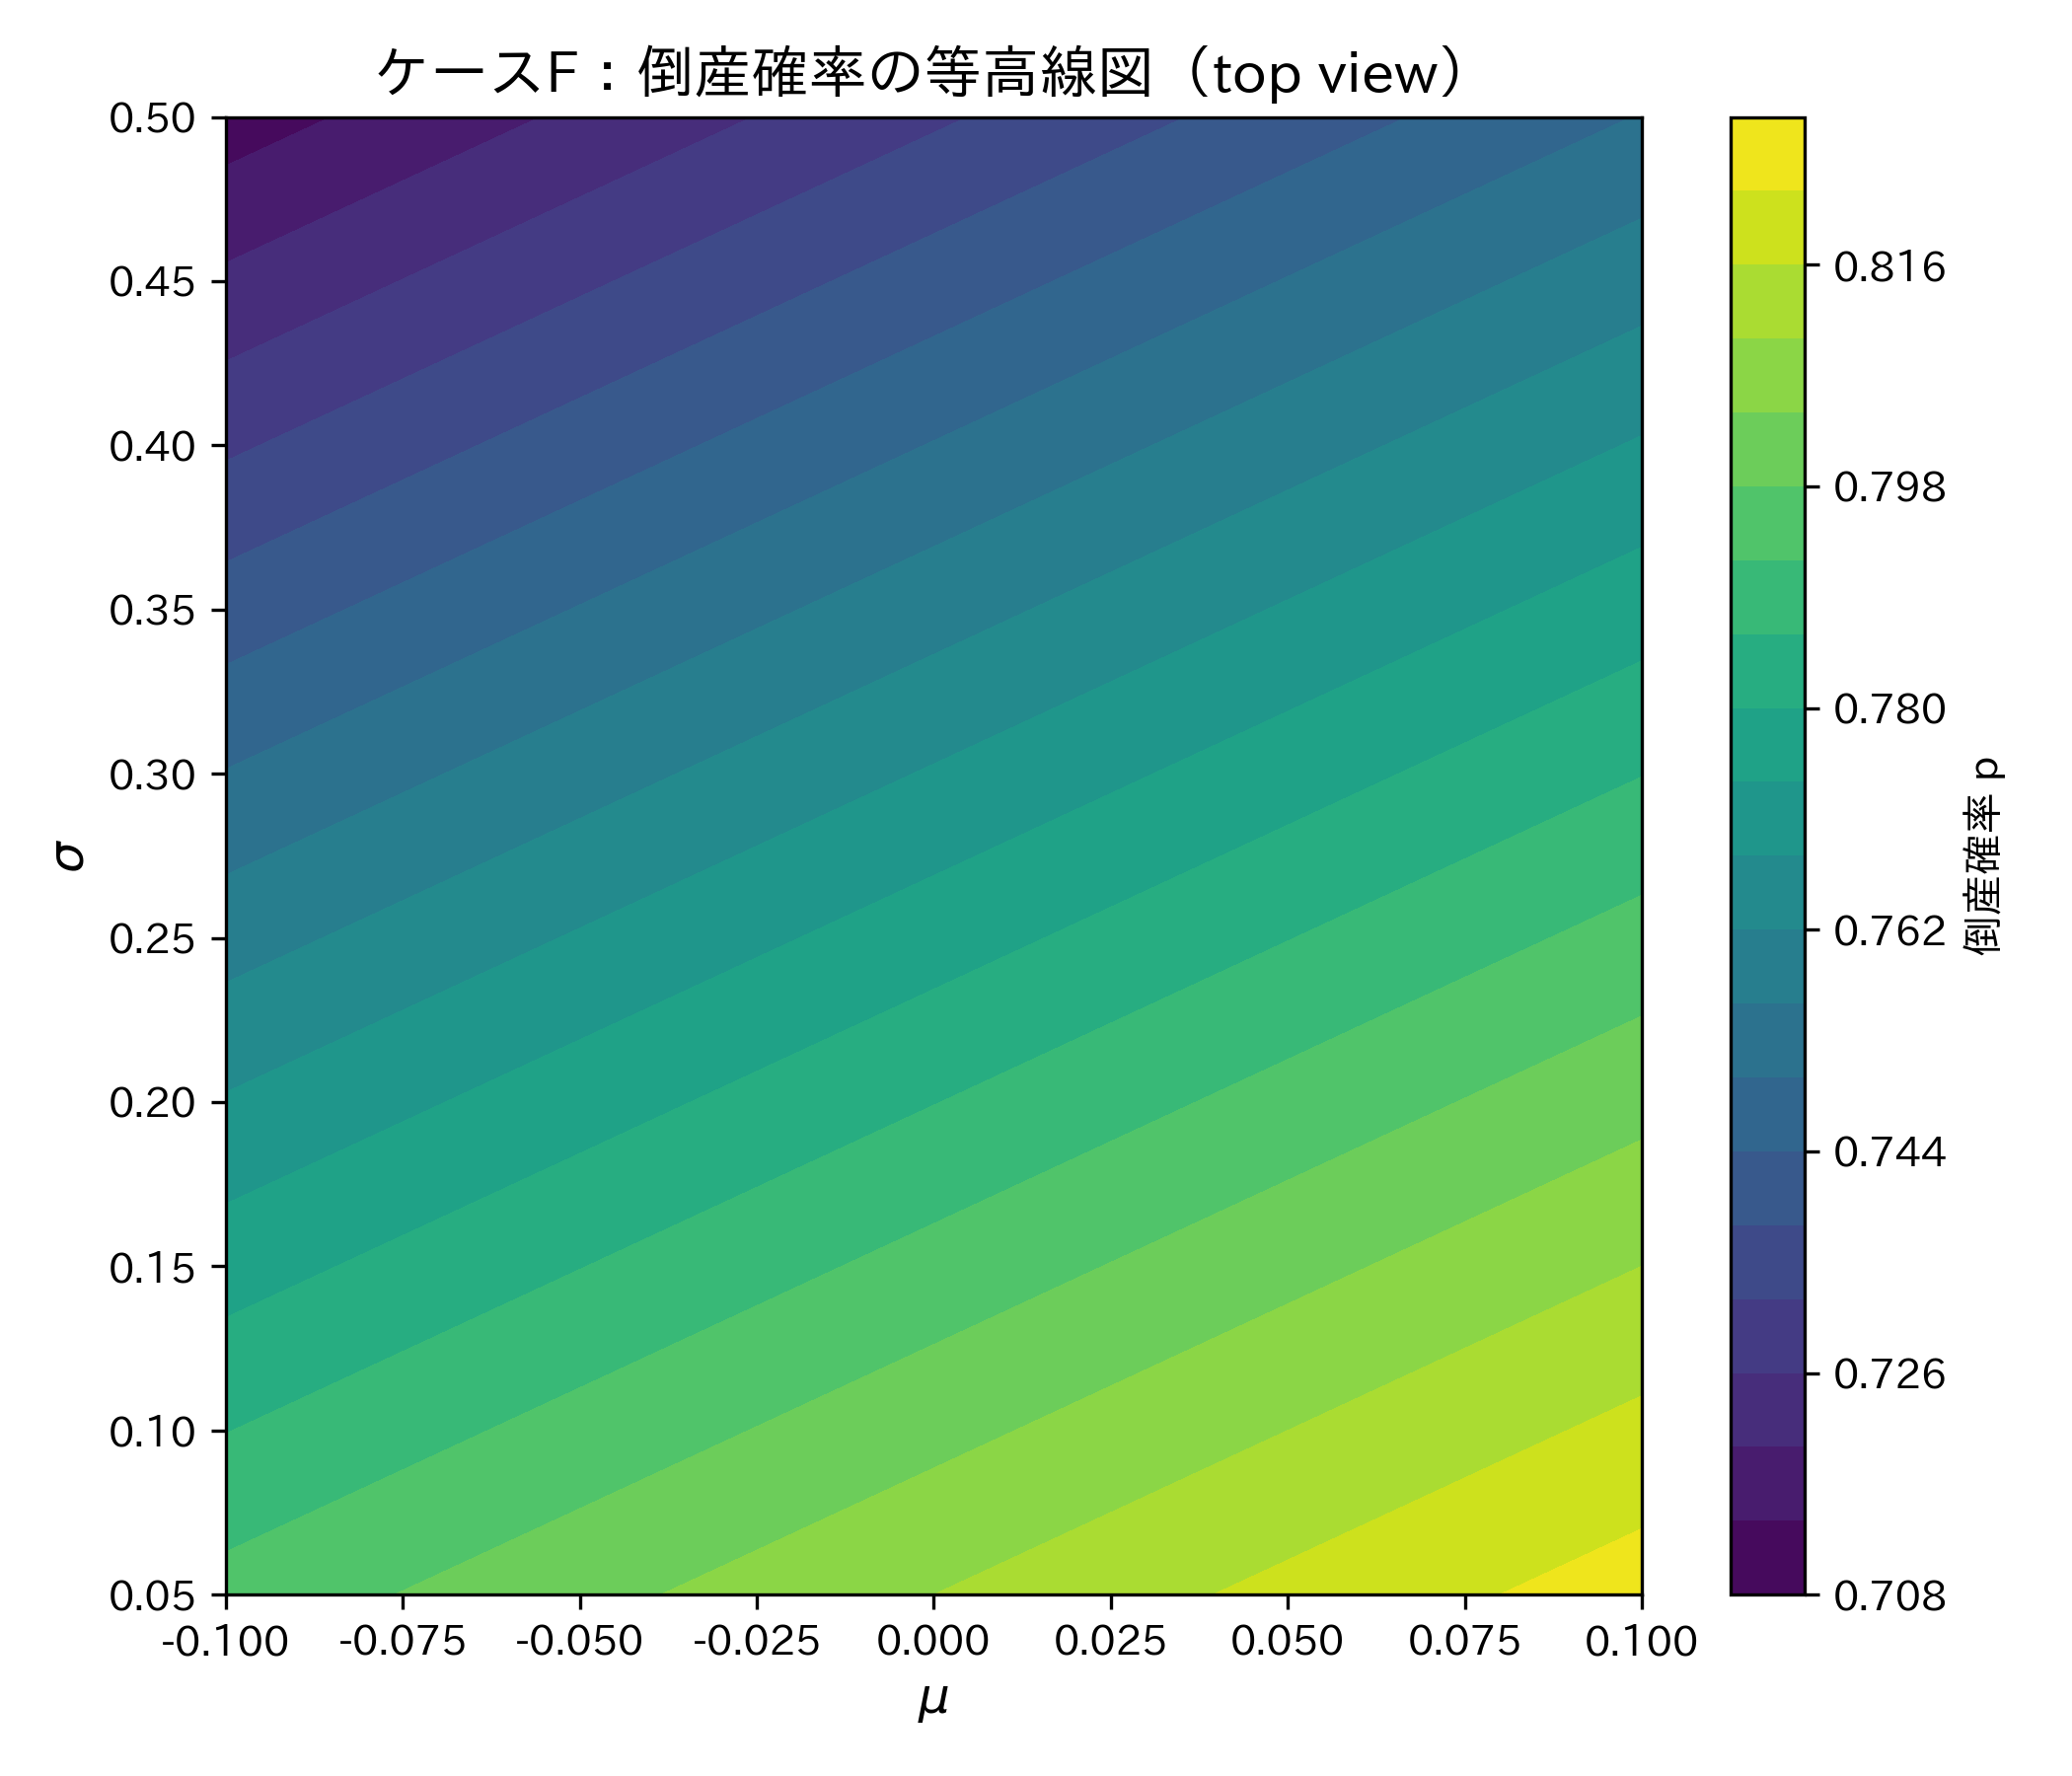
\includegraphics[width=0.75\linewidth]{figures/contour_caseF.png}
    \caption{ケースF（$D=0.5,\ S=2$）：倒産確率の等高線図。
    ケースEと比べて境界線が右へ移動し，
    支援能力の差が倒産リスクを大きく左右することが視覚的に示される。}
\end{figure}

% ------------------------------------------------------------
\section*{C.2 差分図（B−C および F−E）}
\addcontentsline{toc}{section}{C.2 差分図（B−C および F−E）}

本節では，構造的に意味のある 2 組の比較について，
倒産確率の差分 $\Delta p$ を可視化する。
差分図は，支援能力 $S$ と負債比率 $D$ の違いが
倒産確率にどの程度の差を生むかを定量的に示すものである。

\subsection*{C.2.1 大企業 vs 地方電力（ケースB − ケースC）}


\[
\Delta p = p_{\mathrm{B}} - p_{\mathrm{C}}
\]



\begin{figure}[H]
    \centering
    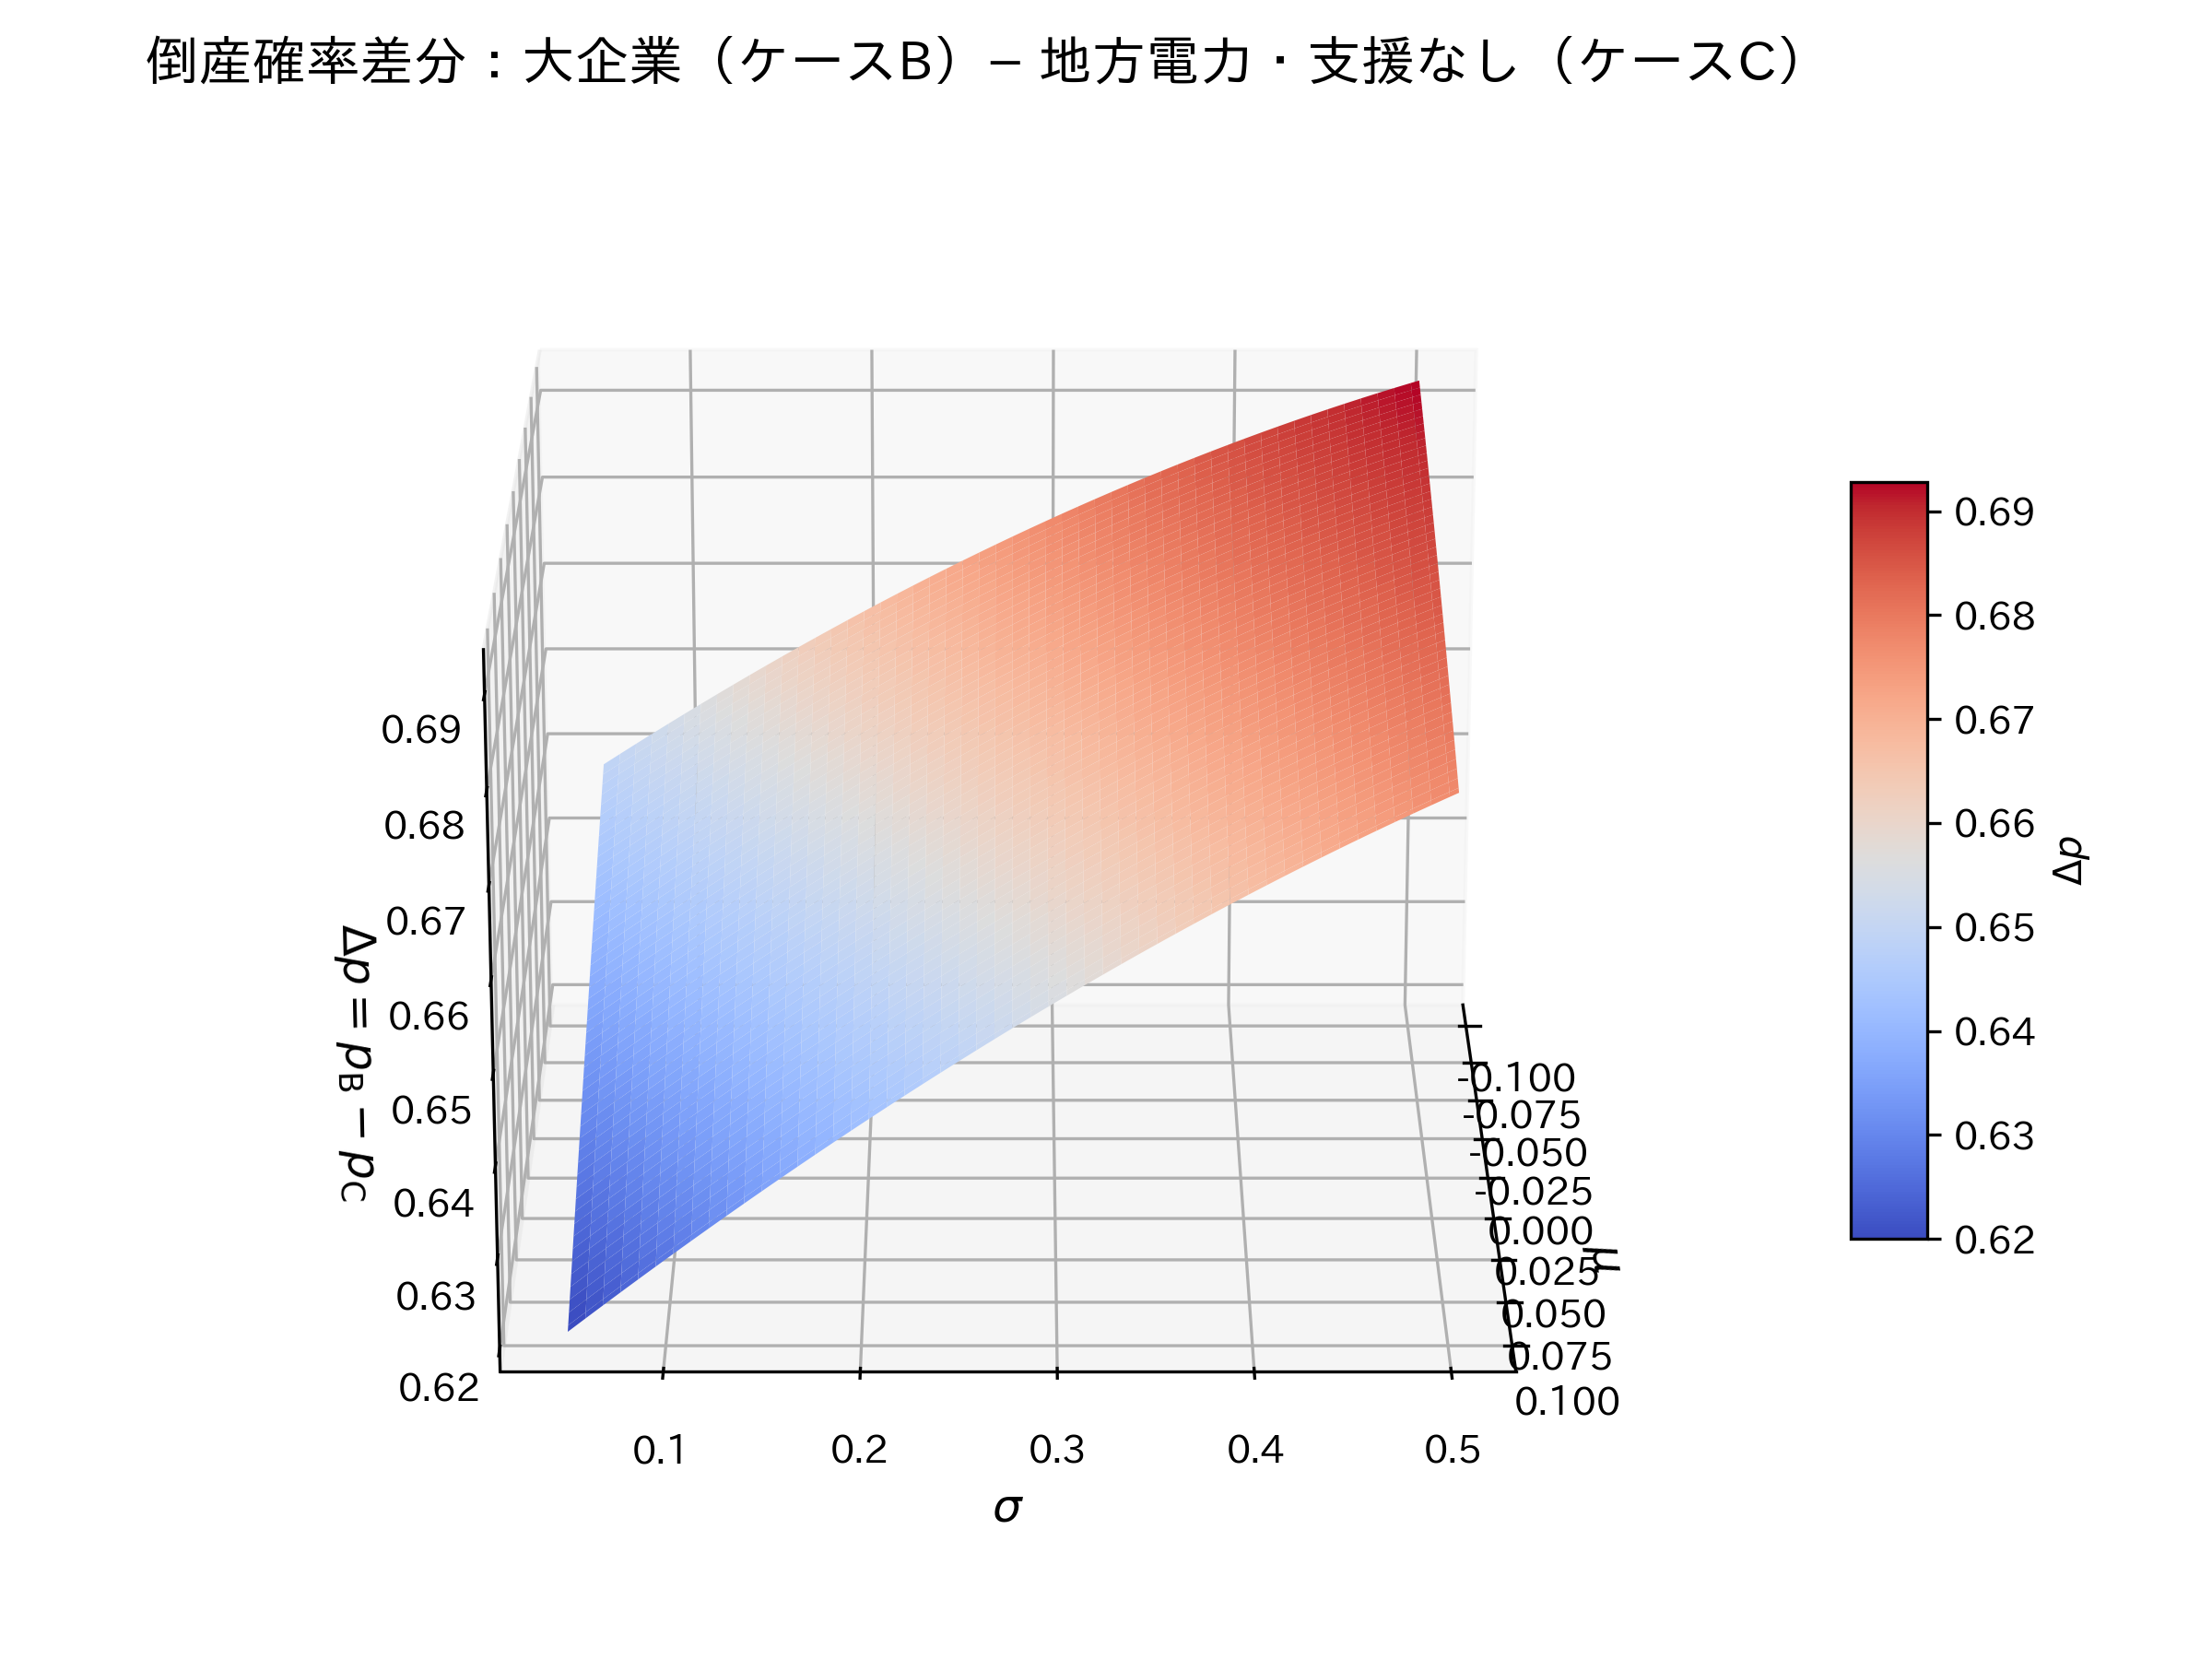
\includegraphics[width=0.75\linewidth]{figures/surface_diff_B_minus_C.png}
    \caption{倒産確率差分：大企業（ケースB）$-$ 地方電力（ケースC）。
    全域で $\Delta p > 0$ となり，支援能力の有無が倒産確率に
    決定的な差を生むことが確認できる。}
\end{figure}

\subsection*{C.2.2 商社系 vs 地域新電力（ケースF − ケースE）}


\[
\Delta p = p_{\mathrm{F}} - p_{\mathrm{E}}
\]



\begin{figure}[H]
    \centering
    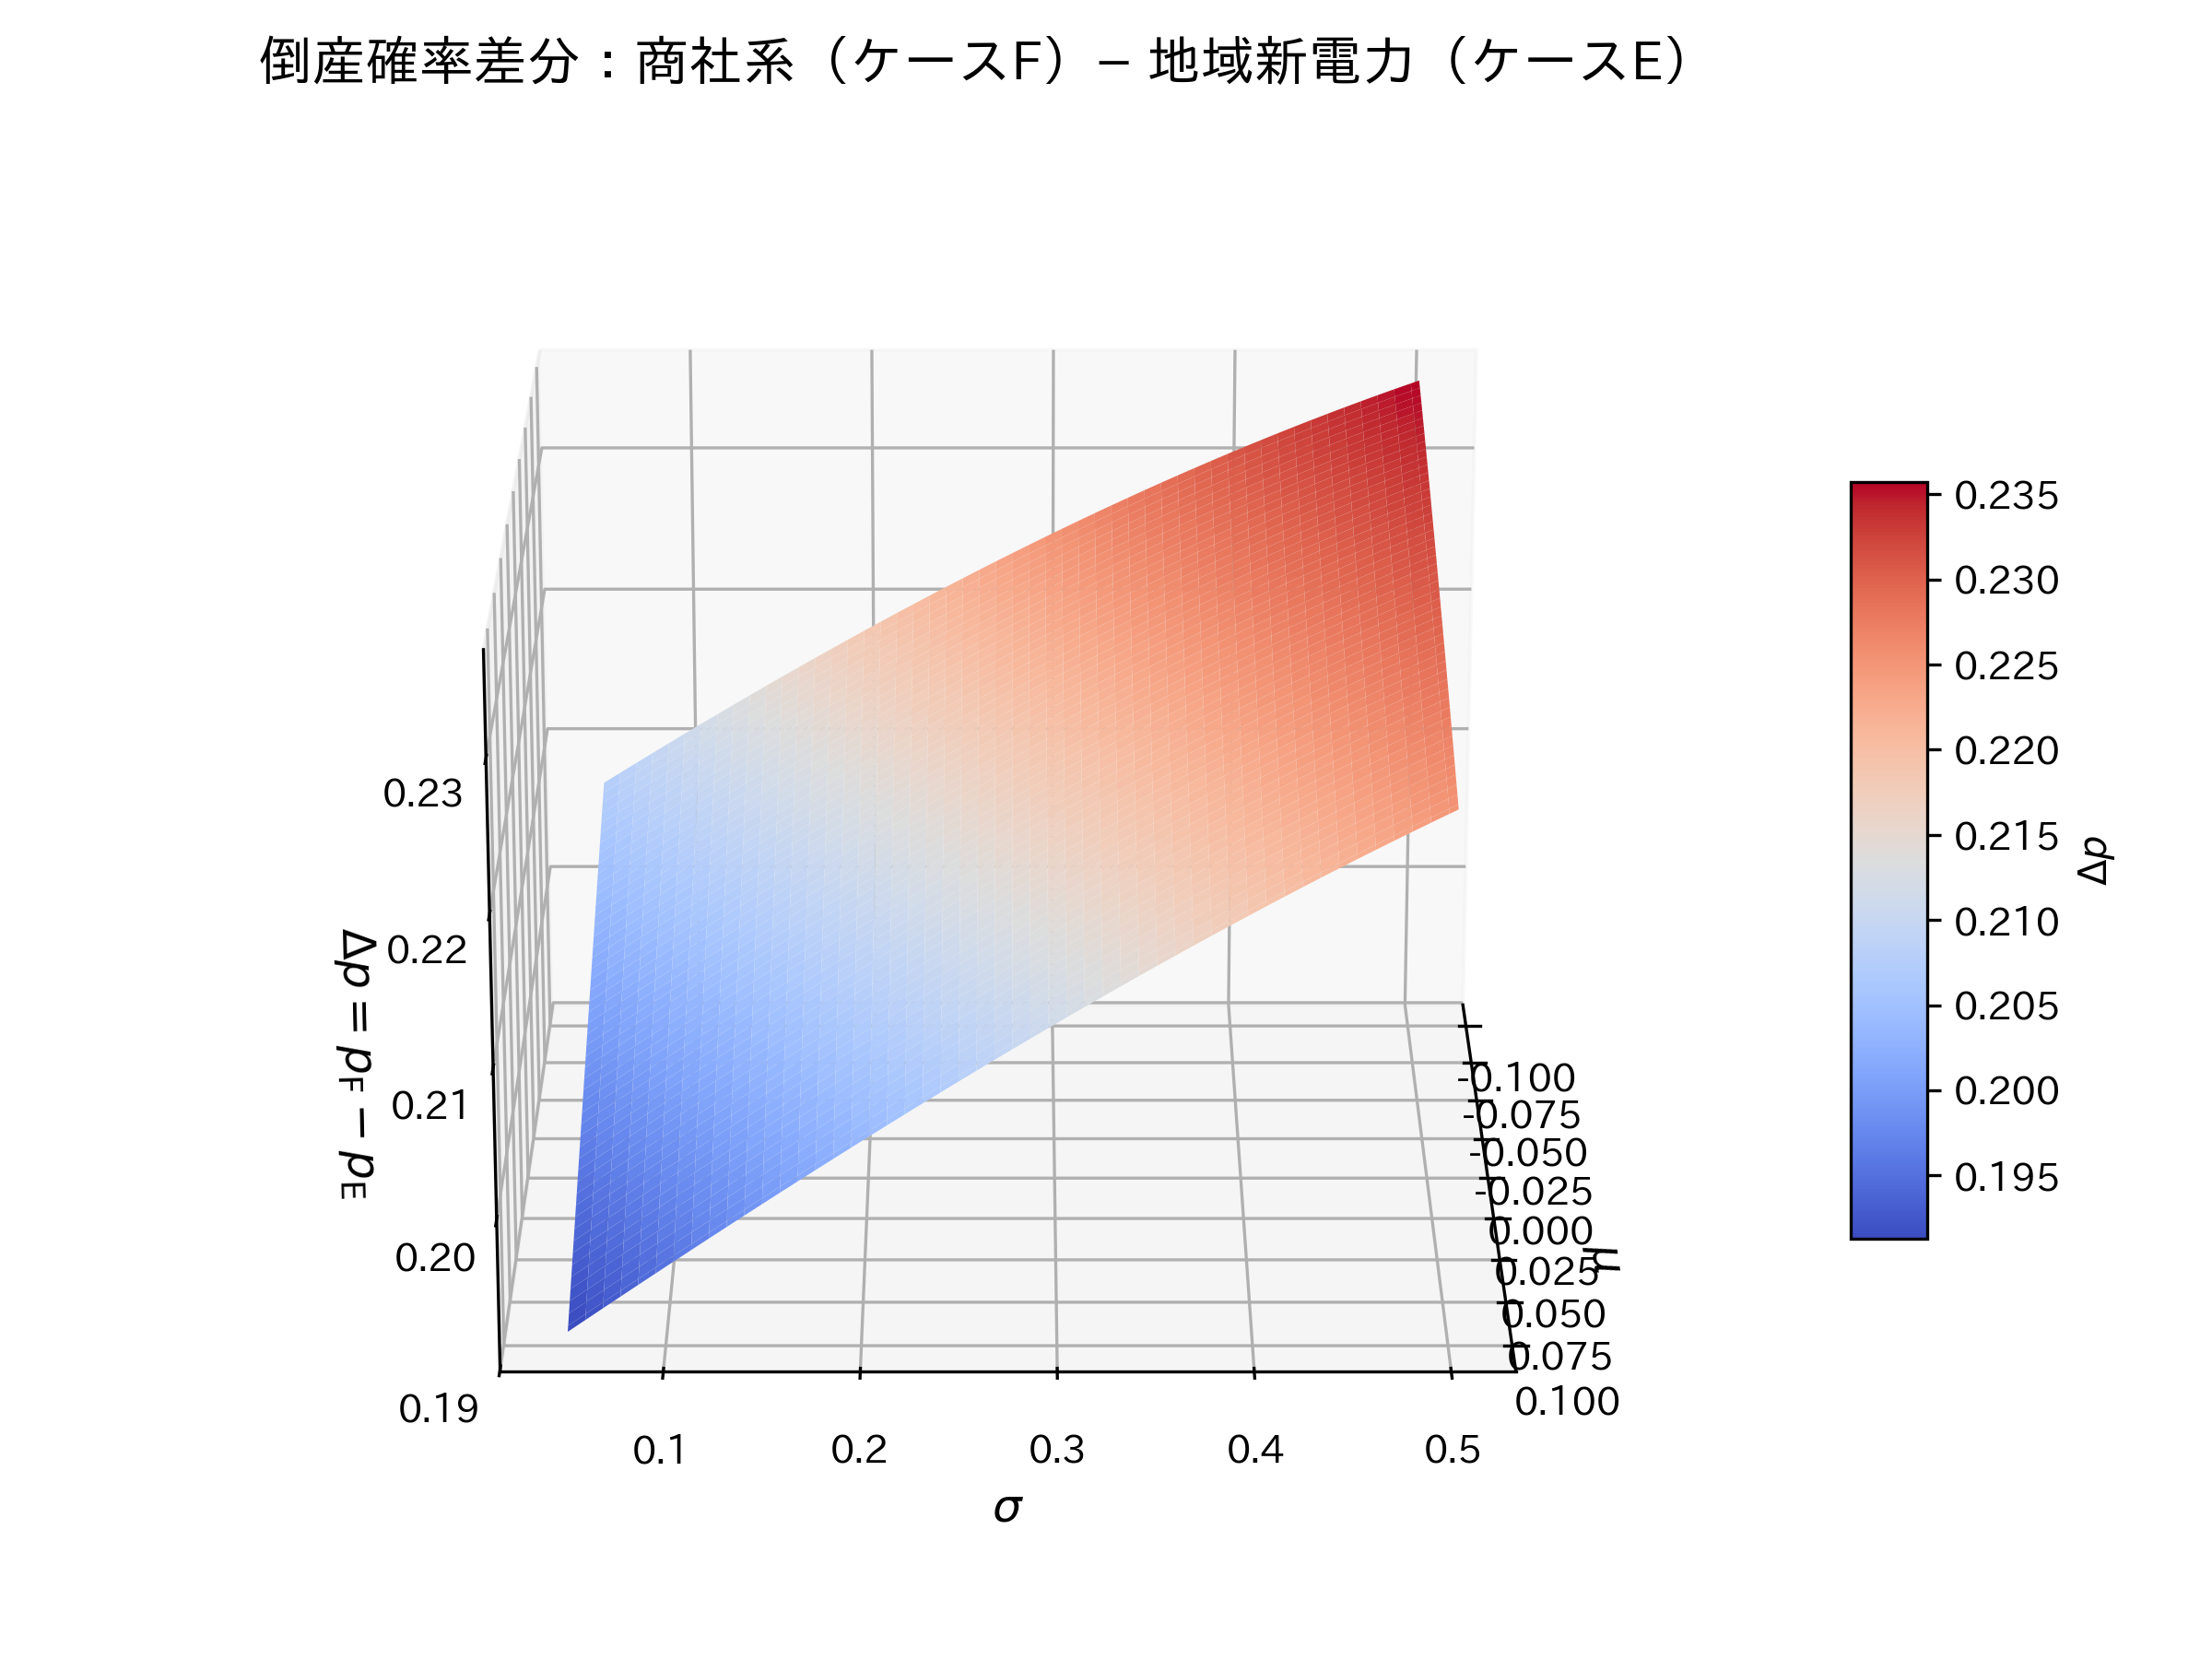
\includegraphics[width=0.75\linewidth]{figures/surface_diff_F_minus_E.png}
    \caption{倒産確率差分：商社系（ケースF）$-$ 地域新電力（ケースE）。
    支援能力 $S$ の差が倒産確率に 0.2〜0.3 程度の差を生み，
    特に $\sigma$ が大きい領域でその効果が最大化する。}
\end{figure}

以上の差分図は，第6章で議論したとおり，
支援能力 $S$ および負債比率 $D$ が倒産確率に与える影響を
視覚的かつ定量的に示すものである。
特に，ケースF−E の比較は，
中規模企業における支援能力の重要性を明確に示している。
